\chapter{Технологическая часть}

В данном разделе рассматривается выбор языка программирования для реализации поставленной задачи, листинги реализации разработанного программного обеспечения и приведены результаты работы ПО.

\section{Выбор языка программирования}

Разработанный модуль ядра написан на языке программирования C \cite{c-language}. Выбор языка программирования С основан на том, что исходный код ядра Linux, все его модули и драйверы написаны на данном языке.

В качестве компилятора выбран gcc \cite{gcc}.

\section{Поиск адреса перехватываемой функции}

Для корректной работы \texttt{ftrace} необходимо найти и сохранить адрес функции, которую будет перехватывать разрабатываемый модуль ядра. 

В старых версиях ядра (в версии ядра 5.7.0 данная функция перестала быть экспортируемой \cite{kallsyms-removed}) найти адрес функции можно было с помощью функции \texttt{kallsyms\_lookup\_name()} -- списка всех символов в ядре, в том числе не экспортируемых для модулей. Так как модуль ядра разрабатывался на системе с версией ядра 5.14.9, воспользоваться данным способом было нельзя. В конечном итоге проблемы была решена с помощью интерфейса \texttt{kprobes} (который был описан в 1.1.3).

Из-за того что данный способ имеет больше накладных расходов, чем поиск с помощью \texttt{kallsyms\_lookup\_name()} (требуется регистрация и удаление \texttt{kprobes} в системе), для версий ядра ниже 5.7.0 поиск адреса производится с помощью \texttt{kallsyms\_lookup\_name()}. Такое реализация стала возможной благодаря директивам условной компиляции \cite{preproc} и специальным макросам 
\texttt{LINUX\_VERSION\_CODE} и \texttt{KERNEL\_VERSION()}. 

Реализация функции \texttt{lookup\_name()}, возвращающей адрес функции перехватываемой функции по её названию, представлена в листинге \ref{lst:lookup_name}.\\

\begin{lstlisting}[label=lst:lookup_name, caption=Реализация функции \texttt{lookup\_name()}, language=c]
#if LINUX_VERSION_CODE >= KERNEL_VERSION(5,7,0)
static unsigned long lookup_name(const char *name)
{
	struct kprobe kp = {
		.symbol_name = name
	};
	unsigned long retval;
	
	ENTER_LOG();
	
	if (register_kprobe(&kp) < 0) {
		EXIT_LOG();
		return 0;
	}
	
	retval = (unsigned long) kp.addr;
	unregister_kprobe(&kp);
	
	EXIT_LOG();
	
	return retval;
}
#else
static unsigned long lookup_name(const char *name)
{
	unsigned long retval;
	
	ENTER_LOG();
	retval = kallsyms_lookup_name(name);
	EXIT_LOG();
	
	return retval;
}
#endif
\end{lstlisting}

\section{Инициализация \texttt{ftrace}}

В листинге \ref{lst:install_hook} представлена реализация функции, которая инициализирует структуру \texttt{ftrace\_ops}.\\

\begin{lstlisting}[label=lst:install_hook, caption=Реализация функции \texttt{install\_hook()}, language=c]
static int install_hook(struct ftrace_hook *hook) {
	int rc;
	
	ENTER_LOG();
	
	if ((rc = resolve_hook_address(hook))) {
		EXIT_LOG();
		return rc;
	}
	
	hook->ops.func = ftrace_thunk; 
	hook->ops.flags = FTRACE_OPS_FL_SAVE_REGS
	| FTRACE_OPS_FL_RECURSION
	| FTRACE_OPS_FL_IPMODIFY;
	
	if ((rc = ftrace_set_filter_ip(&hook->ops, hook->address, 0, 0))) {
		pr_debug("ftrace_set_filter_ip() failed: %d\n", rc);
		return rc;
	}
	
	if ((rc = register_ftrace_function(&hook->ops))) {
		pr_debug("register_ftrace_function() failed: %d\n", rc);
		ftrace_set_filter_ip(&hook->ops, hook->address, 1, 0);
	}
	
	EXIT_LOG();
	
	return rc;
}
\end{lstlisting}

В листинге \ref{lst:remove_hook} представлена реализация отключения перехвата функции.\\

\begin{lstlisting}[label=lst:remove_hook, caption=Реализация функции \texttt{remove\_hook()}, language=c]
static void remove_hook(struct ftrace_hook *hook) {
	int rc;
	
	ENTER_LOG();
	
	if (hook->address == 0x00) {
		EXIT_LOG();
		return;
	}
	
	if ((rc = unregister_ftrace_function(&hook->ops))) {
		pr_debug("unregister_ftrace_function() failed: %d\n", rc);
	}
	
	if ((rc = ftrace_set_filter_ip(&hook->ops, hook->address, 1, 0))) {
		pr_debug("ftrace_set_filter_ip() failed: %d\n", rc);
	}
	
	hook->address = 0x00;
	
	EXIT_LOG();
}
\end{lstlisting}

\section{Функции обёртки}

При объявлении функций обёрток, которые будут запущены вместо перехватываемой функции, необходимо в точности соблюдать сигнатуру. Так, должны совпадать порядок, типы аргументов и возвращаемого значения. Оригинальные описания функций были из исходных кодов ядра Linux. 

В листинге \ref{lst:sys_execve} представлена реализация функции обёртки на примере \texttt{sys\_clone()}.\\

\begin{lstlisting}[label=lst:sys_execve, caption=Реализация функции обёртки, language=c]
static asmlinkage long (*real_sys_clone)(unsigned long clone_flags,
unsigned long newsp, int __user *parent_tidptr,
int __user *child_tidptr, unsigned long tls);

static asmlinkage long hook_sys_clone(unsigned long clone_flags,
unsigned long newsp, int __user *parent_tidptr,
int __user *child_tidptr, unsigned long tls)
{
	update_syscall_array(SYS_CLONE_NUM);
	return real_sys_clone(clone_flags, newsp, parent_tidptr, child_tidptr, tls);
}
\end{lstlisting}

В листинге \ref{lst:update_syscall_array} представлена реализация функции которая обновляет массив, хранящий количество системных вызовов за последние 24 часа.\\

\begin{lstlisting}[label=lst:update_syscall_array, caption=Реализация функции \texttt{update\_syscall\_array()}, language=c]
static DEFINE_SPINLOCK(my_lock);

static void inline update_syscall_array(int syscall_num) {
	ktime_t time;
	
	time = ktime_get_boottime_seconds() - start_time;
	
	spin_lock(&my_lock);
	
	if (syscall_num < 64) {
		syscalls_time_array[time % TIME_ARRAY_SIZE].p1 |= 1UL << syscall_num;
	} else {
		syscalls_time_array[time % TIME_ARRAY_SIZE].p2 |= 1UL << (syscall_num % 64);
	}
	
	spin_unlock(&my_lock);
}
\end{lstlisting}

\section{Примеры работы разработанного ПО}

На рисунках \ref{img:memory_example} - \ref{img:syscalls_example_02} представлены примеры работы разработанного модуля ядра. Для наглядности перехватываются только 18 системных вызовов.

\begin{figure}[h!]
	\begin{center}
		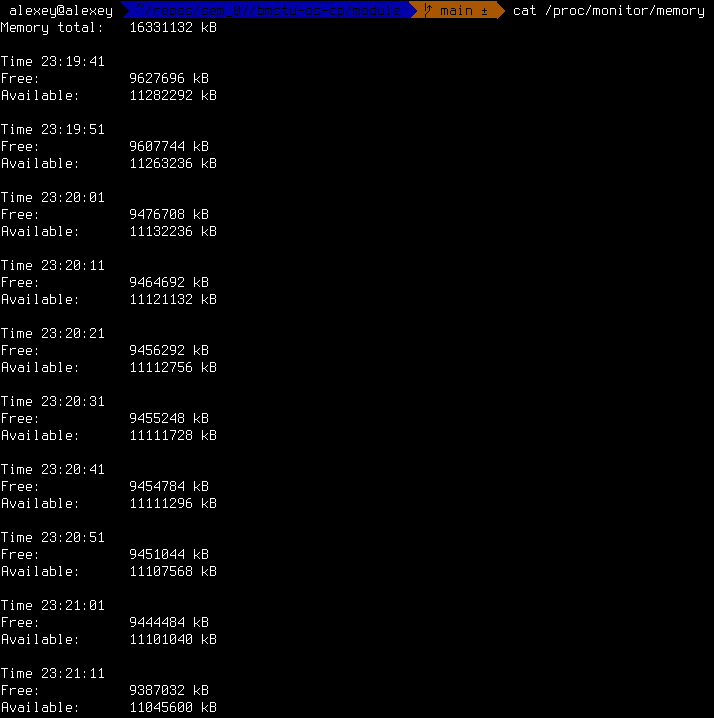
\includegraphics[scale=0.6]{img/memory_example.png}
	\end{center}
	\captionsetup{justification=centering}
	\caption{Информация о оперативной памяти в системе}
	\label{img:memory_example}
\end{figure}

\begin{figure}[h!]
	\begin{center}
		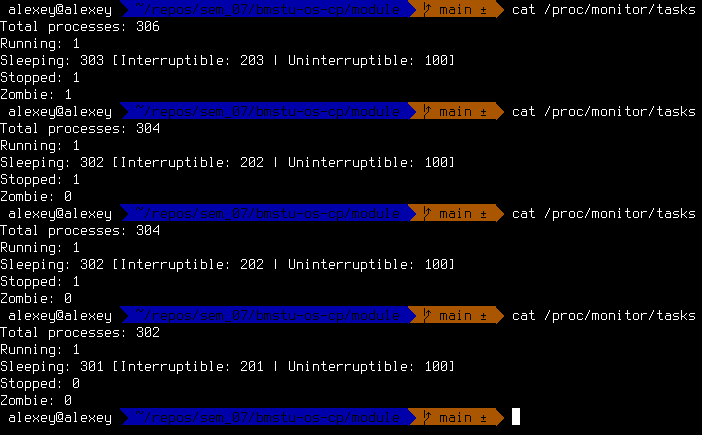
\includegraphics[scale=0.6]{img/tasks_example.png}
	\end{center}
	\captionsetup{justification=centering}
	\caption{Информация о процессах и их состояниях на текущий момент в системе}
	\label{img:tasks_example}
\end{figure}

\begin{figure}[h!]
	\begin{center}
		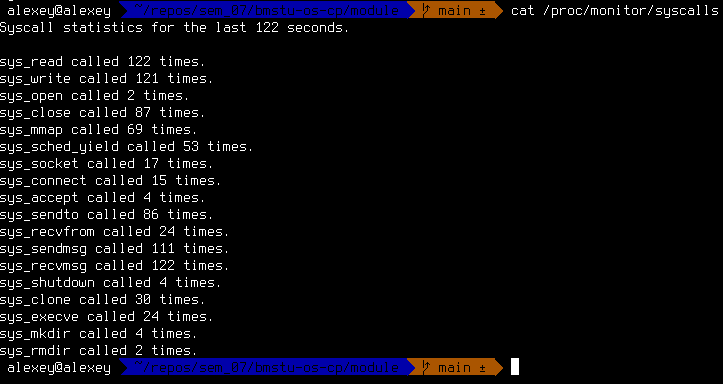
\includegraphics[scale=0.6]{img/syscalls_example_01.png}
	\end{center}
	\captionsetup{justification=centering}
	\caption{Информация о количестве системных вызовов за последние 122 секунды}
	\label{img:syscalls_example_01}
\end{figure}

\begin{figure}[h!]
	\begin{center}
		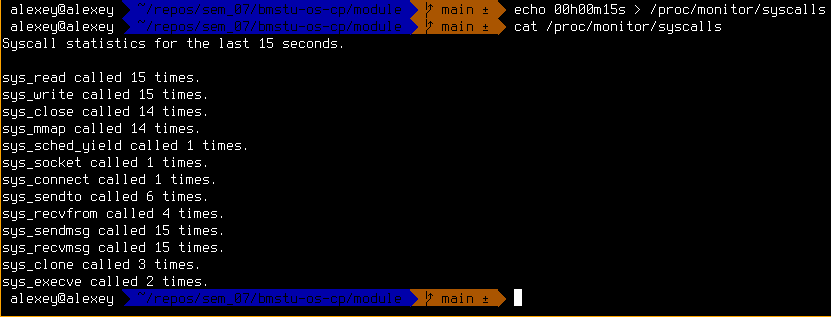
\includegraphics[scale=0.6]{img/syscalls_example_02.png}
	\end{center}
	\captionsetup{justification=centering}
	\caption{Конфигурирование модуля для отображение информации о системных вызовов за последние 15 секунд}
	\label{img:syscalls_example_02}
\end{figure}

\section*{Вывод}

В данном разделе был обоснован выбор языка программирования, рассмотрены листинги реализованного программного обеспечения и приведены результаты работы ПО.